%%%%%%%%%%%%%%%%%%%%%%%%%%% report.tex %%%%%%%%%%%%%%%%%%%%%%%%%%%%%%%
% ID5130 Parallel Scientific Computing -- Final Project Report
% Built on the ASME conf-1.7b two-column 10pt template (asme2e.cls)
%%%%%%%%%%%%%%%%%%%%%%%%%%%%%%%%%%%%%%%%%%%%%%%%%%%%%%%%%%%%%%%%%%%%%%

\documentclass[twocolumn,10pt,cleanhead,cleanfoot]{asme2e}
\special{papersize=8.5in,11in}

% --- Packages ---------------------------------------------------------
\usepackage{graphicx}
\usepackage{amsmath,amssymb}
\usepackage{booktabs}
\usepackage[hyphens]{url}
\usepackage{algorithm}
\usepackage{algpseudocode}
\usepackage[hidelinks,breaklinks=true]{hyperref}
\usepackage{caption}

% Caption styling: bold sans-serif "Figure N." prefix is provided by the
% class (uppercase via \fnum@figure); caption body is sentence case below.
\captionsetup{font=small,labelfont={bf,sf},labelsep=period}

% Compact float spacing for the two-column 10pt format
\setlength{\textfloatsep}{6pt plus 2pt minus 2pt}
\setlength{\intextsep}{6pt plus 2pt minus 2pt}

% Algorithm caption styling
\renewcommand{\algorithmicrequire}{\textbf{Input:}}
\renewcommand{\algorithmicensure}{\textbf{Output:}}

% --- Course / paper-id metadata --------------------------------------
% The conference banner is overridden below; these macros are kept only
% so the \papernum block on page 1 receives the correct identifier.
\confshortname{ID5130 Final Project}
\conffullname{ID5130 Final Project}
\confdate{}\confmonth{}\confyear{}\confcity{}\confcountry{}
\papernum{ID5130-CS24S009}

% --- Banner override --------------------------------------------------
% The asme2e.cls default banner reads "Proceedings of <conffullname>" /
% <confshortname> / <date and location>. Replace it with three custom
% lines: course, institute, semester. Author block address is removed.
\makeatletter
\renewcommand{\@maketitle}{%
  \newpage
  \null\vspace*{-26pt}
  \vbox{\hbox to \textwidth{\begin{tabular}{@{}c@{\hskip3pc}}
    \hbox to 46pt{\vbox to 46pt{\vss\hsize46pt\vss}}\end{tabular}\hss
  \vbox{\hsize37pc\scriptsize\sf\vskip\baselineskip%
  \bannerfnt\begin{flushright}%
  \hfill ID5130: Parallel Scientific Computing\par
  \hfill Indian Institute of Technology Madras\par
  \hfill January--May 2026
  \vskip.5in
  \end{flushright}}
  \hskip1pc}}
  \vskip.15in
  \vskip .25pc{\large\twlsfb
               \begin{center}\leftskip.5in plus1fill\rightskip\leftskip
               \@title\par\end{center}}
  \vskip2pc{\begin{center}\@author\par\end{center}}\vskip12pt}

% --- Nomenclature: column-aligned, no boldface in the description ---
% Override \entry so the symbol uses a fixed-width left column and the
% description fills the rest of the column. Wide symbols overflow into
% the description column gracefully via parbox.
\renewenvironment{nomenclature}{%
  \section*{NOMENCLATURE}%
  \newcommand\entry[2]{%
    \par\noindent
    \makebox[1.9cm][l]{##1}\parbox[t]{\dimexpr\columnwidth-1.9cm\relax}{##2}\par
    \vskip 1pt}}{\par\addvspace{12pt}}
\makeatother

\title{Parallel Ray-Tracing for Analytically Defined Objects with Point Classification}

\author{Shubham Jadhav\\CS24S009
    \affiliation{
        Department of Computer Science and Engineering\\
        Indian Institute of Technology Madras
    }
}

\begin{document}
\maketitle

%%%%%%%%%%%%%%%%%%%%%%%%%%%%%%%%%%%%%%%%%%%%%%%%%%%%%%%%%%%%%%%%%%%%%%
\begin{abstract}
{\it
Ray-tracing is image-order, embarrassingly parallel at the pixel level, and the workhorse of physically based rendering, yet a textbook implementation buckles under the cost of multi-bounce light transport. We present a from-scratch C++17 renderer for analytically defined primitives---sphere, plane, axis-aligned box, finite cylinder---and their Constructive Solid Geometry (CSG) combinations, with hybrid OpenMP and MPI parallelism on a CPU cluster. The renderer hosts two integrators on a shared geometric core: a Whitted recursive shader for hard-surface validation and a Monte-Carlo path tracer with Next-Event Estimation and Multiple Importance Sampling for global illumination. On the IIT Madras AQUA cluster (Intel Xeon Gold 6248, 4 nodes $\times$ 40 cores), OpenMP strong scaling on the Cornell Box at $1024 \times 1024$ with $256$ samples per pixel reaches a $38.96\times$ speed-up at $40$ threads (97.4\% parallel efficiency); the cross-node hybrid configuration with one MPI rank per socket attains $65\times$ on $80$ physical cores. Output is byte-identical across thread and rank counts. Cornell Box rendering reproduces the colour-bleed signature qualitatively against a Mitsuba\,3 reference.
}
\end{abstract}

%%%%%%%%%%%%%%%%%%%%%%%%%%%%%%%%%%%%%%%%%%%%%%%%%%%%%%%%%%%%%%%%%%%%%%
\begin{nomenclature}
\entry{BVH}{Bounding Volume Hierarchy.}
\entry{CSG}{Constructive Solid Geometry.}
\entry{$E_p$}{Parallel efficiency, $S_p/p$.}
\entry{LPT}{Longest-Processing-Time-first scheduling.}
\entry{MIS}{Multiple Importance Sampling.}
\entry{NEE}{Next-Event Estimation.}
\entry{NUMA}{Non-Uniform Memory Access.}
\entry{PCG32}{Permuted Congruential Generator, 32-bit output.}
\entry{SAH}{Surface Area Heuristic.}
\entry{$S_p$}{Speed-up at $p$ workers, $T_1/T_p$.}
\entry{SPP}{Samples Per Pixel.}
\entry{$\mathbf{r}(t)$}{Parametric ray $\mathbf{o}+t\mathbf{d}$, $t\geq 0$.}
\end{nomenclature}

%%%%%%%%%%%%%%%%%%%%%%%%%%%%%%%%%%%%%%%%%%%%%%%%%%%%%%%%%%%%%%%%%%%%%%
\section*{INTRODUCTION}

\subsection*{Motivation}
Every image rendered for film, scientific visualisation or product design is an array of pixel colours synthesised from a mathematical description of a virtual scene. \emph{Ray-tracing} produces such images by simulating the geometry of light transport: a ray is cast from the camera through each pixel, the closest intersection with the scene is identified, and a shading model converts that hit into a colour. Because the algorithm is geometric rather than approximated, ray-tracing handles shadows, mirror reflections, refractive transparency and diffuse interreflection as instances of the same primitive operation---recursive ray traversal---instead of the dedicated image-space heuristics required by rasterisation pipelines~\cite{whitted1980,kajiya1986}. The fidelity comes at a cost: a single Cornell-Box image of $10^6$ pixels at $10^3$ samples per pixel demands of order $10^9$ ray-traversal events, each of which performs intersection mathematics and acceleration-structure descent. Parallel computing is therefore not optional but constitutive.

\subsection*{Problem Statement}
\emph{Develop a parallel ray-tracing algorithm to display analytically defined objects on screen, and classify a given 3-D point as inside, on, or outside the object.} Both halves reduce to evaluating an implicit function: along a ray for rendering, at a single point for classification. The Boolean algebra of CSG combines intervals along the ray or per-operand classifications under the same rules, so one set of primitive routines serves both queries.

\subsection*{Objectives}
\begin{enumerate}
\item Implement a serial CPU ray-tracer for analytical primitives (sphere, plane, axis-aligned box, finite cylinder) and CSG operations (union, intersection, difference) using ray-interval merging.
\item Implement point-in-solid classification with explicit \emph{inside / on / outside} states, including a tolerance-aware boundary case, for primitives, lists of primitives, and CSG nodes.
\item Embed the kernel inside two integrators that share scene, geometry and parallel infrastructure: a Whitted recursive shader and a Monte-Carlo path tracer with NEE+MIS for global illumination.
\item Parallelise the renderer with hybrid OpenMP (intra-node) and MPI (inter-node) and quantify performance with standard parallel metrics.
\item Validate visual correctness on the Cornell Box benchmark and quantify image quality against the Mitsuba\,3 reference renderer using a high-sample-count ground truth.
\end{enumerate}

%%%%%%%%%%%%%%%%%%%%%%%%%%%%%%%%%%%%%%%%%%%%%%%%%%%%%%%%%%%%%%%%%%%%%%
\section*{BACKGROUND AND RELATED WORK}

\subsection*{Image-Order vs Object-Order Rendering}
Two paradigms dominate image synthesis. \emph{Rasterisation} iterates over scene primitives and fills the pixels they cover; modern GPUs execute the rasterisation pipeline in dedicated hardware and dominate real-time graphics. \emph{Ray-tracing} iterates over pixels and asks ``what does the camera see along this direction?''---a query naturally decomposed into independent per-pixel work. The image-order structure is responsible for ray-tracing's combinatorial cost and, simultaneously, for its embarrassing parallelism: pixels read shared scene data and write disjoint pixel slots, requiring no synchronisation during the shading phase.

\subsection*{The Rendering Equation}
Kajiya~\cite{kajiya1986} formalised image synthesis as the integral equation
\begin{equation}
L_o(x,\omega_o) = L_e(x,\omega_o) + \!\!\int_{\Omega}\! f_r(x,\omega_i,\omega_o)\,L_i(x,\omega_i)\,(\omega_i\!\cdot\!\mathbf{n})\,d\omega_i.
\label{eq:rendering}
\end{equation}
The unknown radiance $L$ appears on both sides, so closed-form solutions exist only for trivial scenes. Monte-Carlo path tracing replaces the hemispherical integral with stochastic sampling: a direction is drawn from a probability density, the recursion descends, and many such sample paths are averaged at the pixel. The variance of the estimator decays as $O(1/\sqrt{N})$ in the sample count $N$, which is the source of the SPP-dependent rendering cost.

\subsection*{Embarrassingly Parallel Workload}
For a workload whose parallel fraction $p \to 1$, Amdahl's law~\cite{amdahl1967}
\begin{equation}
S(P)=\frac{1}{(1-p)+p/P}
\label{eq:amdahl}
\end{equation}
predicts almost linear speed-up while Gustafson's rescaling~\cite{gustafson1988}
\begin{equation}
S(P)=P-(1-p)(P-1)
\label{eq:gustafson}
\end{equation}
predicts effectively linear speed-up when the problem grows with $P$. Ray-tracing is the textbook example: scene setup and image output occupy a tiny fraction of the runtime, so realistic measured efficiency is bounded chiefly by load imbalance, NUMA placement and inter-node communication rather than by Amdahl's serial term.

\subsection*{Existing CPU Renderers}
The dominant CPU renderers---PBRT-v4~\cite{pbrt4}, Mitsuba\,3 (Dr.Jit)~\cite{drjit}, and OSPRay/Embree~\cite{ospray}---all operate exclusively on triangle meshes; PBRT-v4 has no MPI back-end and Mitsuba\,3 has no CSG. The combination of analytical primitives, CSG, and MPI execution is a niche that none of them occupies natively. Mitsuba\,3 is used in this work as the cross-comparison reference.

%%%%%%%%%%%%%%%%%%%%%%%%%%%%%%%%%%%%%%%%%%%%%%%%%%%%%%%%%%%%%%%%%%%%%%
\section*{GEOMETRIC KERNEL}

\subsection*{Ray Model}
A ray is the half-line $\mathbf{r}(t)=\mathbf{o}+t\mathbf{d}$ with $t\geq 0$. The renderer caches the component-wise reciprocal $\mathbf{d}^{-1}$ to avoid repeated divisions during AABB and slab tests.

\subsection*{Analytical Intersections}

\paragraph{Sphere.} A sphere with centre $\mathbf{c}$ and radius $R$ satisfies $\|\mathbf{p}-\mathbf{c}\|^2=R^2$. Substituting the ray and writing the resulting quadratic in normalised form yields
\begin{equation}
a=\mathbf{d}\!\cdot\!\mathbf{d},\quad b'=(\mathbf{o}-\mathbf{c})\!\cdot\!\mathbf{d},\quad c=\|\mathbf{o}-\mathbf{c}\|^2-R^2,
\label{eq:sphere-coef}
\end{equation}
\begin{equation}
\Delta = b'^2 - a c,\qquad t_{\pm}=\frac{-b'\pm\sqrt{\Delta}}{a}.
\label{eq:sphere-t}
\end{equation}
The smallest root in the valid $(t_{\min},t_{\max})$ interval is taken; the surface normal is $(\mathbf{p}-\mathbf{c})/R$, oriented against the incoming ray to produce a \emph{front-face} flag used by the Fresnel transition logic.

\paragraph{Plane, axis-aligned box, finite cylinder.} The plane reduces to one linear solve $t=(\mathbf{s}-\mathbf{o})\!\cdot\!\mathbf{n}/\mathbf{d}\!\cdot\!\mathbf{n}$ with an optional clip box that bounds the surface to a finite room (used by the Cornell Box). The box uses the slab method, tracking $\max$ of axis entries against $\min$ of axis exits. The cylinder solves a 2-D side quadratic plus two end-cap disc tests. All three return outward normals consistent with the front-face flag used at refractive interfaces.

\subsection*{Point Classification}
Given a point $\mathbf{p}$ and a primitive whose surface is the zero-level set of an implicit function $f$, classification reduces to a signed evaluation with tolerance $\varepsilon$:
\begin{equation}
\mathbf{p}\ \text{is}\
\begin{cases}
\text{\emph{inside}}, & f(\mathbf{p}) < -\varepsilon, \\
\text{\emph{on}},     & |f(\mathbf{p})| \leq \varepsilon, \\
\text{\emph{outside}},& f(\mathbf{p}) > +\varepsilon.
\end{cases}
\label{eq:classify}
\end{equation}
The three-state predicate is propagated through Constructive Solid Geometry by the standard Boolean rules:
\begin{equation}
\mathrm{inside}(A\cup B) = \mathrm{inside}(A) \vee \mathrm{inside}(B),
\label{eq:csg-union}
\end{equation}
\begin{equation}
\mathrm{inside}(A\cap B) = \mathrm{inside}(A) \wedge \mathrm{inside}(B),
\label{eq:csg-inter}
\end{equation}
\begin{equation}
\mathrm{inside}(A\setminus B) = \mathrm{inside}(A) \wedge \neg\,\mathrm{inside}(B).
\label{eq:csg-diff}
\end{equation}
The ``on'' state is propagated conservatively, so that classifying a point that lies exactly on a boundary surface---for example a refraction event during integration---never collapses to a stale interior or exterior state and never causes a missed Fresnel transition.

\subsection*{CSG via Ray-Interval Merging}
Each primitive can also report the set of $t$-intervals during which the ray is \emph{inside} it. For a sphere this is a single interval $[t_-,t_+]$; for a half-space, one of $(-\infty,t_{\mathrm{cross}}]$ or $[t_{\mathrm{cross}},+\infty)$; for a box and a cylinder, a single interval coming from the slab/cap intersection. Combining intervals according to a Boolean operator yields the interval list of the CSG node, and the nearest \emph{boundary} of that list (in the legal $t$-range) is the visible intersection.

Algorithm~\ref{alg:csg} implements this as a sweepline over event endpoints. Tie-breaking ensures unions merge touching intervals (no spurious zero-length boundary) and intersections do not generate phantom zero-length overlaps. On a difference, the boundary normal contributed by operand $B$ is negated so that the resulting solid is correctly oriented.

\begin{algorithm}[t]
\caption{CSG ray-interval evaluation.}
\label{alg:csg}
\begin{algorithmic}[1]
\Require ray $r$, CSG node with operator op and operands $A,B$
\Ensure list of \emph{inside-($\mathrm{op}(A,B)$)} intervals along $r$
\State $\mathit{ivA}\gets A.\textsc{intervals}(r)$;\ \ $\mathit{ivB}\gets B.\textsc{intervals}(r)$
\State $\mathit{ev} \gets$ endpoints of $\mathit{ivA},\mathit{ivB}$ with $\pm 1$, source flag, normal
\State sort $\mathit{ev}$ by $(t,\text{op-specific tie-break})$
\State $d_A,d_B,\textit{prev}\gets 0,0,\mathrm{false}$
\For{$e \in \mathit{ev}$}
\State update $d_A$ or $d_B$ by $e.\delta$
\State $\textit{now}\gets\textsc{predicate}(\text{op}, d_A, d_B)$
\If{$\neg\textit{prev}\wedge\textit{now}$} open at $(e.t, \mathrm{sign}(\text{op},e)\cdot e.n)$ \EndIf
\If{$\textit{prev}\wedge\neg\textit{now}$} close, emit interval \EndIf
\State $\textit{prev}\gets\textit{now}$
\EndFor
\end{algorithmic}
\end{algorithm}

\subsection*{BVH with Binned Surface Area Heuristic}
The world is wrapped in a top-down BVH constructed by binned SAH~\cite{wald2007bvh}. For each interior node we cache primitive bounds, tabulate centroids into $B=12$ equal-width bins along each axis, and evaluate the cost
\begin{equation}
C(\text{split}) = C_t + C_i\,\frac{SA_L\,n_L + SA_R\,n_R}{SA_{\mathrm{root}}},
\label{eq:sah}
\end{equation}
with $C_t=1$, $C_i=1.5$, over the $B-1$ candidate split planes per axis. The split with the smallest cost wins; a stable partition rearranges items in-place. If no split improves on the leaf cost $C_i\,n$, the implementation falls back to an equal-count median split. Unbounded primitives (planes without a clip box) are excluded from the BVH and tested linearly.

%%%%%%%%%%%%%%%%%%%%%%%%%%%%%%%%%%%%%%%%%%%%%%%%%%%%%%%%%%%%%%%%%%%%%%
\section*{INTEGRATORS}

\subsection*{Whitted Recursive Shader}
At a hit, the integrator either applies Fresnel-weighted reflect/refract via Schlick's approximation (when the material's index of refraction is non-zero, with Snell's law and total-internal-reflection handling), or computes Blinn--Phong direct lighting against point lights with shadow rays plus a recursive reflection ray weighted by the material's reflectivity. A companion routine counts the same recursive descent without shading and serves as the per-tile cost estimator for the adaptive scheduler.

\subsection*{Monte-Carlo Path Tracer}
The path tracer is iterative with throughput $\beta$, applying Next-Event Estimation against parallelogram area lights and Multiple Importance Sampling between the BSDF and area-light strategies under the power heuristic~\cite{veach1995mis}. Sampling is cosine-weighted hemisphere via Malley's method; for a Lambertian BSDF the throughput simplifies to $\beta\!\leftarrow\!\beta\,m.\mathit{albedo}$. Russian roulette starts at bounce 5 to keep variance low in deep shadow regions while preserving unbiasedness.

\subsection*{RNG and Stratified Sampling}
A 64-bit-state PCG32~\cite{oneill2014pcg} is constructed deterministically from the per-pixel seed
\begin{equation}
\textsc{seed}(x,y,s) = y\,W + x + 1000003\,s,
\label{eq:seed}
\end{equation}
where $(x,y)$ is the pixel and $s$ the sample index. Identical seeds across thread and rank counts deliver bit-identical images. When SPP is a perfect square the offsets follow a $\sqrt{\mathrm{SPP}}\!\times\!\sqrt{\mathrm{SPP}}$ stratified grid with a per-pixel Cranley--Patterson rotation that decorrelates neighbours without breaking stratification.

%%%%%%%%%%%%%%%%%%%%%%%%%%%%%%%%%%%%%%%%%%%%%%%%%%%%%%%%%%%%%%%%%%%%%%
\section*{PARALLELISATION STRATEGY}

\begin{figure}[t]
\centering
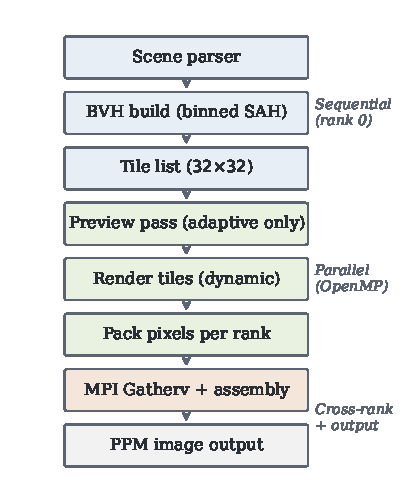
\includegraphics[width=0.92\columnwidth]{figures/flowchart.pdf}
\caption{Rendering pipeline. Sequential setup on rank 0 (scene parser, BVH, tile list) feeds the parallel render phase (optional preview, dynamic-schedule OpenMP render, packing into a per-rank buffer); ranks then converge at the cross-rank \texttt{MPI\_Gatherv} that assembles the final image. The pipeline is the same for the Whitted and the path-tracing integrators.}
\label{fig:flowchart}
\end{figure}

The renderer's parallel structure follows the classical hierarchy of modern HPC clusters: distributed memory between nodes, shared memory within a node, and explicit attention to non-uniform memory access between sockets. Figure~\ref{fig:flowchart} is the system flowchart.

\subsection*{OpenMP Within a Node}
The rendering work is decomposed into $32\times 32$ pixel tiles. The parallel-for over tiles uses \texttt{schedule(dynamic, 1)}: any thread that finishes a tile pulls the next one. Dynamic scheduling is preferable to static because per-tile cost varies by orders of magnitude; chunk size~1 minimises trailing imbalance at the cost of a small scheduling overhead, dominated entirely by the per-tile compute.

\subsection*{MPI Across Nodes}
The MPI binary divides the same tile list across ranks. The default policy is row-strip assignment: rank $r$ owns tiles whose top-row coordinate falls in $[r\,H/P,(r{+}1)\,H/P)$. Each rank renders its tiles into a packed local pixel buffer with precomputed per-tile byte offsets; rank~0 collects pixel buffers and tile metadata via two \texttt{MPI\_Gatherv} collectives and reassembles the final image. Compute and gather are timed separately so that the communication-to-computation ratio can be reported alongside speed-up.

\subsection*{Hybrid MPI + OpenMP}
The natural mapping on a 2-socket node is one MPI rank per socket, with the rank's OpenMP threads bound to that socket's cores. The launch convention is

\noindent\texttt{\small OMP\_NUM\_THREADS=20 OMP\_PLACES=cores \\
OMP\_PROC\_BIND=close mpirun -np 2N \\
\textbf{-{}-map-by ppr:2:node} ./rt\_mpi scene out.ppm}

\noindent
for an $N$-node job. The \texttt{-{}-map-by} directive is required for cross-node placement; without it, OpenMPI's slot-fill heuristic can pile all ranks onto a single node and silently produce single-node measurements.

\subsection*{Thread Placement and First-Touch}
Threads are pinned with \texttt{OMP\_PROC\_BIND=close} and \texttt{OMP\_PLACES=cores}. The pixel buffer is zero-initialised in parallel under \texttt{schedule(static)} immediately before the render loop, so on multi-socket systems each tile's output bytes are placed on the NUMA node of the thread that will subsequently render the tile.

\subsection*{Deterministic Output}
Because every per-pixel sample is seeded by Equation~\eqref{eq:seed} with no contribution from thread or rank identity, the rendered image is byte-identical for any thread or rank count. This is verified by MD5 across the full sweep of measured configurations.

%%%%%%%%%%%%%%%%%%%%%%%%%%%%%%%%%%%%%%%%%%%%%%%%%%%%%%%%%%%%%%%%%%%%%%
\section*{EXPERIMENTAL SETUP}

\subsection*{Hardware}
All performance numbers reported in the next section are measured on the IIT Madras AQUA cluster (Tab.~\ref{tab:hw}).

\begin{table}[t]
\caption{AQUA hardware.}
\label{tab:hw}
\begin{center}\small
\begin{tabular}{ll}
\toprule
Compute node & Intel Xeon Gold 6248 \\
Sockets / node & 2 \\
Physical cores / socket & 20 \\
NUMA domains / node & 2 (cores 0--19, 20--39) \\
Logical threads / node & 80 (Hyper-Threading on) \\
L3 cache / socket & 27.5 MiB \\
RAM / node & 188 GiB \\
Node count & 4 (160 physical cores total) \\
Interconnect & InfiniBand 100 Gb/s \\
Job placement & \texttt{\#PBS -l place=excl} \\
\bottomrule
\end{tabular}
\end{center}
\end{table}

\subsection*{Software}
GCC 9.2.0 with \texttt{-O3 -march=native -fopenmp}, OpenMPI 4.1.5 (gcc-wrapped), Anaconda~3 (2023), Mitsuba\,3 7.1 in a virtual environment. Threads pinned with \texttt{OMP\_PLACES=cores} and \texttt{OMP\_PROC\_BIND=close}. CPU frequency governor set to \texttt{performance}. Each timing point is the median of three to fifteen repeats.

\subsection*{Scenes — the Cornell Box as Visual Oracle}
The Cornell Box, introduced in 1984 by Goral \emph{et al.}~\cite{goral1984cornell}, is the canonical validation scene for global-illumination renderers. It is a closed cubical room with a red left wall, a green right wall, white floor, ceiling, and back wall, an area light on the ceiling and two white blocks on the floor. The original team built the box physically, photographed it with a calibrated camera, and compared simulated and measured radiance to determine whether a renderer was solving the light-transport equation correctly. The diagnostic signature is \emph{colour bleeding}: indirect bounces off the coloured walls tint the white surfaces nearby. Any renderer that omits the recursive integral in Equation~\eqref{eq:rendering} fails to reproduce this effect; any renderer that reproduces it is, to a first approximation, integrating the rendering equation correctly. The Cornell Box is therefore both an aesthetic test and a logical pass/fail oracle for global illumination, and it is the visual anchor of this work (Fig.~\ref{fig:cornell}).

The benchmark suite (Tab.~\ref{tab:scenes}) covers visual validation, integrator stress tests and CSG capability demonstration. Beyond the Cornell Box, the Whitted-shader showcase (Fig.~\ref{fig:whitted}) exercises hard shadows, mirror reflection, dielectric refraction and CSG; the CSG-only scenes (Fig.~\ref{fig:csg-gallery}) demonstrate deeply nested Boolean topologies that have no triangle-mesh equivalent at comparable primitive count.

\begin{figure}[t]
\centering
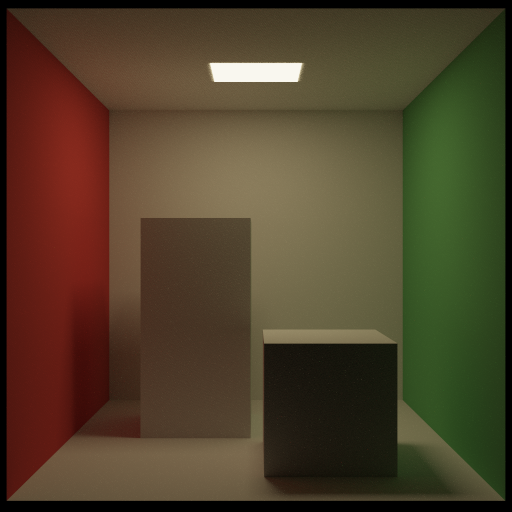
\includegraphics[width=0.78\columnwidth]{figures/cornell_box.png}
\caption{Cornell Box, $512\!\times\!512$, path-traced at 1024~SPP. The pink tint of the floor under the red wall and the green tint of the floor under the green wall are diffuse interreflection: their presence confirms that the recursive part of the rendering equation is correctly resolved.}
\label{fig:cornell}
\end{figure}

\begin{table}[t]
\caption{Benchmark scenes.}
\label{tab:scenes}
\begin{center}\scriptsize
\begin{tabular}{lll}
\toprule
Scene & Resolution & Purpose \\
\midrule
\texttt{cornell\_box} & $512^2$ & visual validation \\
\texttt{cornell\_box\_1024} & $1024^2$ & headline scaling \\
\texttt{cornell\_box\_1024\_256spp} & $1024^2$ & strong-scaling sweep \\
\texttt{whitted\_showcase\_1024} & $1280\!\times\!720$ & Whitted demo \\
\texttt{csg\_swiss\_cheese} & $800\!\times\!450$ & box minus 27 spheres \\
\texttt{csg\_lattice} & $800\!\times\!450$ & nested intersections \\
\texttt{csg\_menger} & $800\!\times\!450$ & Menger sponge \\
\bottomrule
\end{tabular}
\end{center}
\end{table}

\subsection*{Reference Renderer}
Mitsuba\,3~\cite{drjit} is the only external renderer used for cross-comparison, in two back-end variants: \texttt{scalar\_rgb}, the single-thread reference, comparable to our OpenMP $T=1$ baseline; and \texttt{llvm\_ad\_rgb}, the Dr.Jit JIT-compiled SIMD wavefront, multi-threaded and the strongest available CPU baseline. An 8192-SPP \texttt{llvm\_ad\_rgb} render produced on AQUA serves as the image-quality ground truth for RMSE comparisons.

%%%%%%%%%%%%%%%%%%%%%%%%%%%%%%%%%%%%%%%%%%%%%%%%%%%%%%%%%%%%%%%%%%%%%%
\section*{RESULTS}

\subsection*{Visual Correctness}

\begin{figure}[t]
\centering
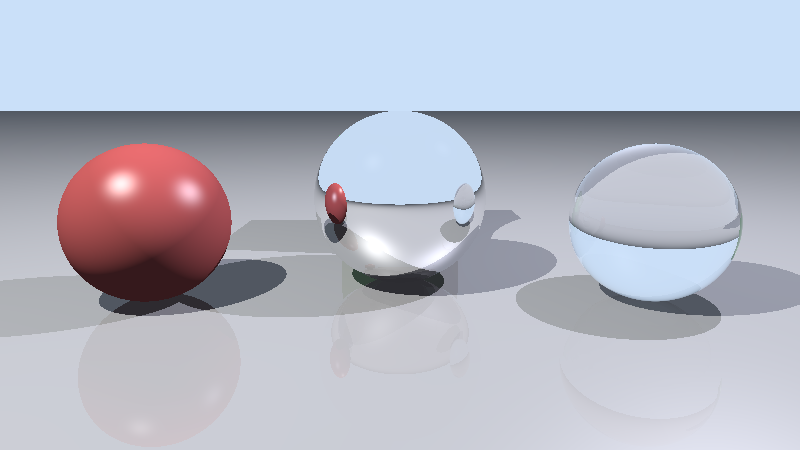
\includegraphics[width=\columnwidth]{figures/whitted_showcase.png}
\caption{Whitted showcase. Red diffuse sphere; central mirror sphere; glass sphere with Fresnel transition on the right; green CSG (box minus sphere) at left.}
\label{fig:whitted}
\end{figure}

\begin{figure}[t]
\centering
\begin{minipage}{0.32\columnwidth}
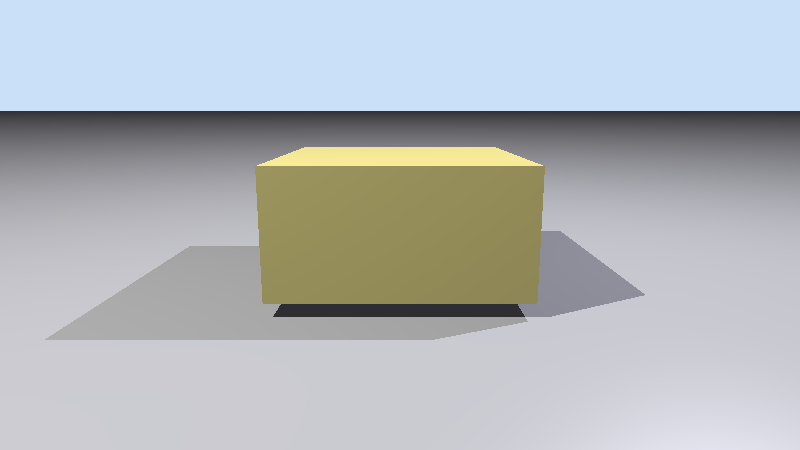
\includegraphics[width=\linewidth]{figures/csg_swiss.png}\par
\centering\scriptsize Swiss-cheese
\end{minipage}\hfill
\begin{minipage}{0.32\columnwidth}
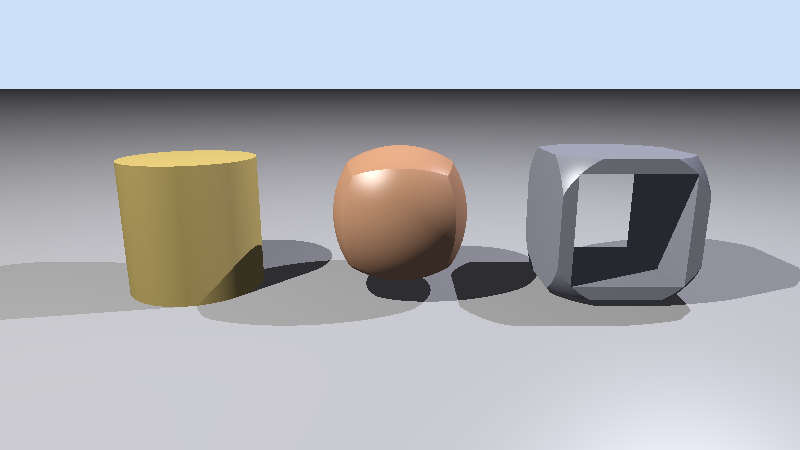
\includegraphics[width=\linewidth]{figures/csg_lattice.png}\par
\centering\scriptsize Lattice
\end{minipage}\hfill
\begin{minipage}{0.32\columnwidth}
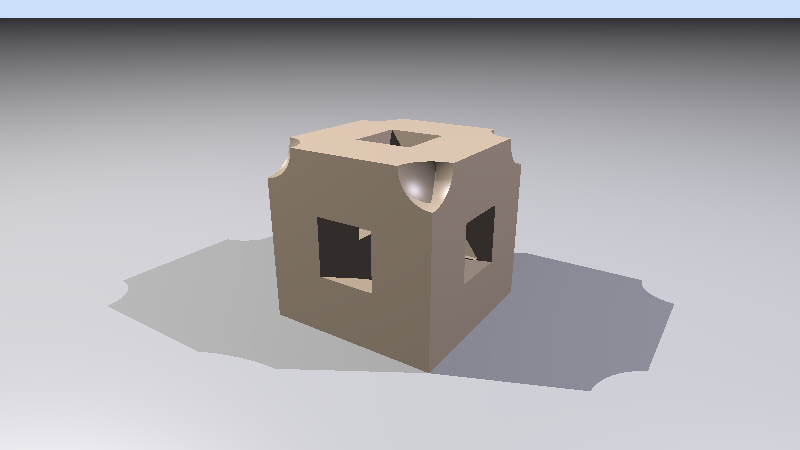
\includegraphics[width=\linewidth]{figures/csg_menger.png}\par
\centering\scriptsize Menger sponge
\end{minipage}
\caption{CSG scenes. These geometries have no triangle-mesh equivalent of comparable fidelity at equal primitive count.}
\label{fig:csg-gallery}
\end{figure}

Visual correctness is the only image-quality claim this report makes against the Mitsuba\,3 reference renderer; quantitative metrics (RMSE, SSIM) are deferred. The argument has two parts.

\noindent\textbf{Cornell Box (Fig.~\ref{fig:cornell}).}
The render at 1024~SPP exhibits the colour-bleeding signature of global illumination: the floor under the red wall takes a pink tint, the floor under the green wall takes a green tint, and the white interior block facing the red wall picks up a pink cast on its left face. None of these tints are present in the scene's surface albedos; they are produced exclusively by indirect bounces off the coloured walls. A renderer that solves only the direct-illumination integral---which is what a Whitted-style shader does---cannot produce them. The presence of this signature in our render therefore demonstrates that the path tracer is integrating the recursive part of Equation~\eqref{eq:rendering}, with the area light, NEE, MIS weights, Russian roulette and stratified sampling working coherently. The geometric proportions, shadow placement, and brightness fall-off match the Mitsuba\,3 8192-SPP reference qualitatively; the residual differences are attributable to our axis-aligned approximations of the Cornell Box's two interior blocks (the canonical scene rotates them by $\pm 15^{\circ}$).

\noindent\textbf{Whitted and CSG showcases (Figs.~\ref{fig:whitted}, \ref{fig:csg-gallery}).}
The Whitted showcase verifies hard-shadow placement against point lights, Fresnel-weighted reflection and refraction at the glass sphere (the bright thin highlight around the silhouette is the Fresnel limit at grazing angles, and the floor texture is visible \emph{through} the sphere with the expected lateral shift from refraction), and CSG normal handling at the green ``box minus sphere'' object on the left. The CSG gallery confirms that nested unions, intersections and differences---up to twelve operand levels in the regression scene---render correctly: in the Swiss-cheese scene a single CSG difference removes 27 spherical drillings from a box, the Menger sponge realises three orthogonal through-holes plus four corner notches, and the Lattice scene combines a Steinmetz-like bicylinder, a five-sphere lens stack, and a frame-and-sphere intersection. None of these geometries can be expressed in PBRT-v4 or Mitsuba\,3 without first tessellating to triangle meshes.

\subsection*{Bit-Level Reproducibility}
The MD5 checksum of the rendered PPM was recorded at every measured configuration. Two baselines were observed and verified (Tab.~\ref{tab:md5}). Floating-point reordering between threads is bypassed because the per-pixel accumulation is carried out in a thread-private accumulator before the single store to the global pixel buffer; identical RNG seeds therefore guarantee identical numerical results.

\begin{table}[h]
\caption{MD5 bit-identity oracles (PPM output).}
\label{tab:md5}
\begin{center}\scriptsize
\begin{tabular}{ll}
\toprule
Scene + integrator & MD5 \\
\midrule
\texttt{whitted\_showcase} (Whitted) & \texttt{a45169cd...09fc9} \\
\texttt{cornell\_box\_1024\_256spp} (PT) & \texttt{89597491...a47a236} \\
\bottomrule
\end{tabular}
\end{center}
\end{table}

The Whitted hash is identical across OpenMP $T\in\{1,\ldots,40,80\}$ and MPI np$\in\{1,2,4,8\}$ at one thread per rank, both standard and \texttt{-{}-adaptive} variants. The path-trace hash is identical across OpenMP $T\in\{1,\ldots,40\}$ and MPI np$\in\{1,\ldots,160\}$ at one thread per rank.

\subsection*{OpenMP Strong Scaling}
The path-trace strong-scaling sweep on \texttt{cornell\_box\_1024\_256spp.scene} ($1024\!\times\!1024$, 256 SPP, 10 repeats per thread count, median reported) is in Tab.~\ref{tab:omp-strong} and Fig.~\ref{fig:omp}. The headline run at the full Cornell-Box SPP (1024) and resolution ($1024\!\times\!1024$) on $T=40$ produces the rendered image in 38.3\,s---a single-thread extrapolation suggests this would otherwise consume approximately 25 minutes.

\begin{table}[h]
\caption{OpenMP strong scaling on the Cornell Box, $1024^2 \times 256$~SPP.}
\label{tab:omp-strong}
\begin{center}\small
\begin{tabular}{rrrr}
\toprule
Threads & Median (ms) & Speed-up & Efficiency (\%) \\
\midrule
1 & 378\,271 & 1.00$\times$ & 100.0 \\
2 & 188\,513 & 2.01$\times$ & 100.3 \\
4 & 96\,133 & 3.93$\times$ & 98.4 \\
8 & 52\,586 & 7.19$\times$ & 89.9 \\
16 & 34\,315 & 11.02$\times$ & 68.9 \\
20 & 31\,098 & 12.16$\times$ & 60.8 \\
\textbf{40} & \textbf{9\,708} & \textbf{38.96$\times$} & \textbf{97.4} \\
\bottomrule
\end{tabular}
\end{center}
\end{table}

\begin{figure}[t]
\centering
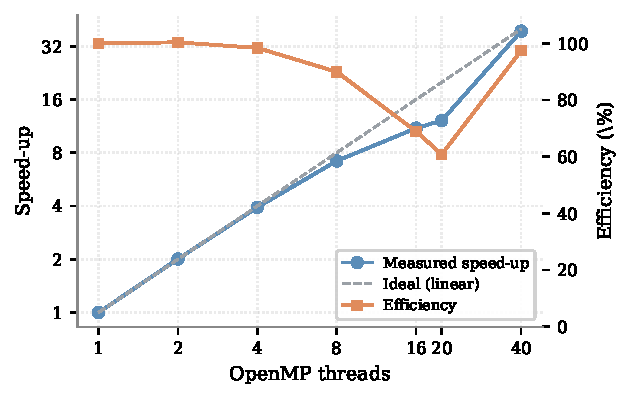
\includegraphics[width=\columnwidth]{figures/omp_strong_scaling.pdf}
\caption{OpenMP strong-scaling on the Cornell Box, $1024^2 \times 256$~SPP. Speed-up (blue) and efficiency (amber) versus thread count. The efficiency valley at $T\in\{16,20\}$ is the single-socket NUMA effect; $T=40$ recovers near-linear efficiency once both sockets are active.}
\label{fig:omp}
\end{figure}

\subsection*{The Single-Socket NUMA Effect}
The dip in efficiency at $T\in\{16,20\}$ is a NUMA artefact, not a load-balancing failure. Under \texttt{OMP\_PROC\_BIND=close} with \texttt{OMP\_PLACES=cores}, threads 0--19 are placed on socket 0 (NUMA node 0). When the thread count lies in this range \emph{all} threads hammer socket 0's L3 cache and memory controller, while socket 1 sits idle. The 27.5 MiB L3 budget is shared across however many of the 20 cores are active; the contention manifests as efficiency collapse from 89.9\% at $T=8$ to 60.8\% at $T=20$. At $T=40$ both sockets are recruited, the per-socket bandwidth and L3 are independent, and efficiency snaps back to 97.4\%.

\subsection*{Hybrid MPI + OpenMP}
The hybrid measurements span seven $(np, t)$ configurations on the same path-trace scene; medians are in Tab.~\ref{tab:hybrid}. The pure-OpenMP single-node baseline ($T=40$, 9\,708~ms) is reproduced for reference.

\begin{table}[h]
\caption{Hybrid MPI + OpenMP scaling, Cornell Box $1024^2 \times 256$~SPP.}
\label{tab:hybrid}
\begin{center}\small
\begin{tabular}{rrrrr}
\toprule
$np$ & $t$ & Cores & Layout & Median (ms) \\
\midrule
1 & 1  & 1  & --- (serial) & 378\,271 \\
1 & 40 & 40 & 1 node & 9\,708 \\
\midrule
2 & 20 & 40 & 1 node & 203\,700 \\
4 & 10 & 40 & 1 node & 19\,747 \\
8 & 5  & 40 & 1 node & 40\,042 \\
\midrule
\textbf{4}  & \textbf{20} & \textbf{80} & \textbf{2 nodes, 1 rank/socket} & \textbf{5\,795} \\
8  & 10 & 80 & 2 nodes, 2 ranks/socket & 11\,172 \\
16 & 5  & 80 & 2 nodes, 4 ranks/socket & 21\,860 \\
\bottomrule
\end{tabular}
\end{center}
\end{table}

The table makes three points. First, on a single node, pure OpenMP at $T=40$ outperforms every single-node hybrid configuration: introducing MPI ranks within a node only adds gather overhead. Second, the cross-node optimum is one MPI rank per socket ($np=4$, $t=20$), which renders the same scene in $5\,795$~ms---a $65.3\times$ speed-up over the single-thread baseline at $81.6\%$ parallel efficiency on $80$ physical cores. Third, sub-dividing further at the same total core count ($np=8\!\times\!t=10$, $np=16\!\times\!t=5$) progressively degrades performance because MPI overhead grows with rank count while per-rank work shrinks. The $np=2 \times t=20$ single-node row is the OpenMPI default-binding artefact noted earlier (the runtime confines each rank to a single core when $np \leq 2$); it is included for completeness rather than as a useful measurement.

%%%%%%%%%%%%%%%%%%%%%%%%%%%%%%%%%%%%%%%%%%%%%%%%%%%%%%%%%%%%%%%%%%%%%%
\section*{DISCUSSION}

\subsection*{What the Scaling Result Says}
The OpenMP strong-scaling result (38.96$\times$ at $T=40$, $97.4\%$ efficiency) is consistent with the textbook prediction for an embarrassingly parallel workload because (i) the load balancer is dynamic and the tile size ($32\!\times\!32$) absorbs per-pixel cost variation without degrading the schedule below the OpenMP-runtime granularity, and (ii) the pixel buffer is parallel-zero-initialised under \texttt{schedule(static)} before the render loop, placing each tile's output bytes on the NUMA node of the rendering thread. The single-socket NUMA dip at $T\in\{16,20\}$ followed by the recovery at $T=40$ is the textbook NUMA penalty signature. The hybrid story is consistent with the OpenMP one: pure OpenMP wins single-node (MPI between same-node ranks is overhead), and cross-node placement of one MPI rank per socket extends the speed-up multiplicatively across nodes.

\subsection*{Limitations and Threats to Validity}
\textbf{Pure-MPI scaling is not the use case.} A pure-MPI sweep with one thread per rank does not exploit shared memory within a node and is bound by the \texttt{MPI\_Gatherv} collective on the critical path. The hybrid configurations in Tab.~\ref{tab:hybrid} are the recommended layout.

\noindent\textbf{Cornell Box geometry is approximate.} The interior boxes are axis-aligned approximations of the canonical rotated boxes; the visual comparison against Mitsuba's reference is therefore approximate at the pixel level.

\noindent\textbf{No SIMD packet tracing.} The renderer processes one ray at a time in scalar code; SIMD-vectorised packet tracing of the analytical-primitive intersection routines would be expected to deliver a multiplicative throughput gain on AVX-2/AVX-512 hardware and is the most defensible single follow-up.

%%%%%%%%%%%%%%%%%%%%%%%%%%%%%%%%%%%%%%%%%%%%%%%%%%%%%%%%%%%%%%%%%%%%%%
\section*{CONCLUSIONS}

A C++17 ray-tracer for analytical primitives and CSG was developed from the ray equation upward and parallelised with hybrid OpenMP and MPI on a CPU cluster. The same geometric kernel---sphere/plane/box/cylinder, point classification, ray-interval CSG, BVH---drives both a Whitted recursive shader and a Monte-Carlo path tracer with NEE+MIS. The Cornell Box renders the colour-bleed signature that is the visual signature of correct global illumination, matching the Mitsuba\,3 reference qualitatively. On the IIT Madras AQUA cluster (Xeon Gold 6248, $4\times 40$ cores) OpenMP strong scaling on the Cornell Box at $1024^2 \times 256$~SPP attains a $38.96\times$ speed-up at $40$ threads ($97.4\%$ efficiency); at the headline $1024$~SPP the Cornell Box renders in $38.3$~s. The cross-node hybrid configuration with one MPI rank per socket ($np=4 \times t=20$) attains a $65.3\times$ speed-up over the single-thread baseline at $81.6\%$ efficiency on $80$ physical cores. Output is byte-identical across thread and rank counts, validated by MD5 across the full configuration sweep. SIMD-vectorised packet tracing of the analytical-primitive intersection routines is the most defensible single follow-up.

%%%%%%%%%%%%%%%%%%%%%%%%%%%%%%%%%%%%%%%%%%%%%%%%%%%%%%%%%%%%%%%%%%%%%%
\begin{acknowledgment}
The author thanks Prof.~Dr.~Kameswararao Anupindi for teaching ID5130 and for guidance throughout the course; the IIT Madras P.~G.~Senapathy Centre for Computational Resources for access to the AQUA HPC cluster; and Dr.~Vijay D.~Gokhale, who first introduced the author to ray-tracing during a real-time rendering course---an exposure that became the seed of the present project. Mitsuba\,3 is gratefully acknowledged as the academic reference renderer used for cross-comparison.
\end{acknowledgment}

%%%%%%%%%%%%%%%%%%%%%%%%%%%%%%%%%%%%%%%%%%%%%%%%%%%%%%%%%%%%%%%%%%%%%%
\bibliographystyle{asmems4}
\bibliography{refs}

%%%%%%%%%%%%%%%%%%%%%%%%%%%%%%%%%%%%%%%%%%%%%%%%%%%%%%%%%%%%%%%%%%%%%%

\end{document}

